%
%  $Description: Orientação para autores e exemplo de documento em LaTeX 2.09$
%
%  $Autor: Gabriel P. Silva $
%  $Data: 15/04/2009 15:20:59 $
%  $Revisão: 1.0 $
%

\documentclass[10pt,twocolumn]{article}
\usepackage{wscad2009}
\usepackage{times}
\usepackage[portuges]{babel}
%\usepackage[latin1]{inputenc}

% Se você estiver utilizando uma distribuição Linux Fedora ou Mandriva
% Use utf8
\usepackage[utf8]{inputenc}
% Para incluir gráficos e figuras use o pacote abaixo
%\usepackage[dvips]{graphicx}

\usepackage[pdftex]{graphicx}
\DeclareGraphicsExtensions{.pdf,.jpeg,.png, .jpg}

\usepackage{verbatim}
\usepackage{url}

\hyphenation{op-tical net-works semi-conduc-tor ca-tas-tro-fi-cas fa-lhas di-fe-ren-te-men-te mo-di-fi-ca-do to-le-ran-tes vo-lu-me re-qui-si-tos es-ca-lo-na-men-to crackers to-le-ran-te hamming exis-tir ope-ra-cio-nal ou-tros exem-plo }

%-------------------------------------------------------------------------
\pagestyle{empty}
%-------------------------------------------------------------------------
\begin{document}

\title{Técnica de Proteção de Bytecodes para Processador Java em Tecnologia CMOS}

%\author{Blind review
\author{Jardel Silveira (jardel@lesc.ufc.br), David Viana (david@lesc.ufc.br) \\ Helano Castro (helano@lesc.ufc.br), Alexandre Coelho (alexandre@lesc.ufc.br) \\ Jarbas Silveira (jarbas@lesc.ufc.br) \\
Universidade Federal do Ceará \\ LESC (http://www.lesc.ufc.br) \\ Fortaleza, CE, Brasil  %\\ jardel@lesc.ufc.br\\
% Para autores que pertencem a uma mesma instituição,
% omita as seguintes linhas até o último ``}''.
% Neste caso use $^{1}$ para colocar um sobrescrito nos autores e
% respectivos endereços de e-mail
% Para adicionar autores com endereços diferentes coloque um ``\and'',
% como no caso do segundo autor a seguir:
%\and
%Segundo Autor\\
%Instituição2\\
%Primeira lina do endereço da instituição2\\ Segunda linha do endereço da instituição2\\
%SegundoAutor@institucao2.edu.br\\
}

\maketitle
\thispagestyle{empty}

\begin{abstract}
	%Sistemas embarcados de tempo real têm severas restrições de garantia de funcionamento, tais como: re\-qui\-si\-tos temporais, consumo, peso e vo\-lu\-me total ocupado.  Considerando o projeto de circuitos integrados, para atingir o nível de confiabilidade requerido por esses sistemas, podem-se usar processos de fabricação de circuitos integrados específicos ou aplicar técnicas de garantia de funcionamento na fase de projeto do circuito integrado. Além disso, no \emph{software} e no nível sistêmico, ou seja, na integração dos componentes eletrônicos em uma placa de circuito impresso, também é possível aplicar técnicas para aumentar a confiabilidade destes sistemas.
	%Os circuitos integrados manufaturados através de processos específicos têm alto custo devido ao pequeno volume de produção destes, (Melhor a vírgula que o ponto) portanto, é preferível fazer o projeto de um circuito integrado tolerante a falhas e poder manufaturá-lo usando um processo que esteja no estado da arte.
	%Do ponto de vista do desenvolvimento de \emph{software}, os recursos fornecidos pela linguagem de programação utilizada para programar tais sistemas podem influenciar no nível de confiabilidade do sistema. O uso de linguagens com um alto nível de abstração, como {J}ava, pode diminuir a ocorrência de erros de programação, reduzindo, assim, o número de falhas não antecipadas, introduzidas durante o desenvolvimento. O \emph{soft core} JOP (\emph{Java Optimized Processor}) para FPGAs (\emph{Field Programmable Gate Array}) é uma implementação otimizada da máquina virtual Java, no âmbito do \emph{hardware},   para aplicações de tempo real.
	%Neste trabalho, propomos uma técnica de projeto de \emph{hardware} para o \emph{soft core} JOP, que detecta e corrige erros na área destinada ao código da memória SRAM (\emph{Static Random Access Memory}). A ocorrência da falha é percebida no nível sistêmico através de uma exceção, característica esta disponível na linguagem {J}ava. A técnica proposta aumenta a confiabilidade do sistema e mantêm as características de tempo real do \emph{soft core} JOP.
  O \emph{soft core} JOP (\emph{Java Optimized Processor}) para FPGAs (\emph{Field Programmable Gate Array}) é uma implementação otimizada da máquina virtual Java em \emph{hardware},   para aplicações de tempo real. No entanto, este processador não contempla em sua arquitetura técnicas de tolerância a falhas. O trabalho descrito neste artigo é parte de um esforço maior para tornar o processador JOP um processador tolerante a falhas. Neste artigo, apresentamos os resultados da aplicação de uma técnica de tolerância a falhas, proteção de memória através de ECC (\emph{Error Correction Code}), no \emph{soft core} JOP, que detecta e corrige erros na área destinada ao código da memória SRAM (\emph{Static Random Access Memory}). A ocorrência da falha é percebida no nível sistêmico através de uma exceção, característica esta disponível na linguagem {J}ava. Este artigo apresenta resultados inovadores na medida em que não existem registrados na literatura outro processador Java de tempo real e tolerante a falhas.
\end{abstract}
\section{Introdução}
	Os sistemas eletrônicos de tempo real embarcados em missões espaciais estão sujeitos aos elevados níveis de radiação existentes no espaço. Por isso, tais sistemas estão sujeitos a falhas causadas pelas colisões de partículas altamente energizadas contra estruturas nanométricas de silício presentes nos circuitos integrados modernos.

	Particularmente para circuitos integrados contendo blocos de memória SRAM, a principal conseqüência destas colisões é a ocorrência de SEUs (\emph{single event upsets}), que são  a inversão permanente do valor de um bit. Existem fábricas especializadas na produção de circuitos integrados tolerantes à radiação. No entanto, devido ao pequeno volume de produção desses circuitos integrados, os mesmos têm preços elevados. Portanto, é muito importante garantir tolerância à radiação no âmbito do projeto do circuito integrado, independentemente do processo de fabricação, pois isto reduz os custos do sistema e permite utilizar os mais modernos processos de fabricação existentes.

	Devido ao tamanho reduzido e a alta frequência de operação dos circuitos eletrônicos digitais modernos, os mesmos estão cada vez mais sucetíveis a ruído. Por isso, problemas antes somente encontrados em sistemas submetidos a radiações com intensidade similar à espacial, hoje são enfrentados em sistemas operando em ambiente terrestre. Aplicações seguras constituem outro exemplo em ambiente terrestre que requerem técnicas de tolerância a falhas, pois falhas em sistemas seguros podem ser exploradas por \emph{crackers} para descobrir chaves secretas armazenadas na memória interna de um circuito integrado \cite{RSAFaultAttack}.

	Diante desse cenário, percebe-se cada vez mais a necessidade da utilização de técnicas de tolerância a falhas não somente em sistemas embarcados em missões espaciais, mas também nos sistemas terrestres. Dentre alguns exemplos dessas aplicações terrestres podemos citar a indústria automobilística, bancos e outras aplicações cujos requisitos temporais e de alta disponibilidade são prioritários para o correto funcionamento do sistema.

	Notavelmente, a linguagem de programação {C} é atualmente a mais utilizada para desenvolvimento de \emph{software} para sistemas embarcados, tanto para o sistema ope\-ra\-cio\-nal quanto para a aplicação. Isto pode ser facilmente demonstrado por uma análise dos compiladores comerciais disponíveis para os processadores modernos de sistemas embarcados.

	Usualmente, o sistema operacional é responsável por funções de suporte a tempo real, gerenciamento de memória e comunicação inter-processos. Tais recursos são disponibilizados para a aplicação por meio de chamadas de sistema (\emph{system calls}) \cite{TanenbaumModernOS} e de uma API (\emph{Application Program Interface}).

	O uso de uma linguagem de alto nível de abstração traz benefícios do ponto de vista do desenvolvimento do sistema, tais como diminuir a probabilidade de erros de codificação e a redução do tempo de desenvolvimento de um sistema \cite{RTProgLang}. {J}ava é uma linguagem de alto nível muito utilizada e com grande suporte  para o desenvolvimento de sistemas \emph{standalone}. Além do alto nível de abstração, a linguagem {J}ava traz no seu núcleo (Máquina Virtual {J}ava) recursos comumente implementados em nível de sistema operacional, tais como comunicação inter-processo e escalonamento de tarefas.

	Em uma implementação tradicional de sistemas embarcados de tempo real, baseada em um processador de uso geral e um sistema operacional de tempo real, essas vantagens têm um custo elevado em termos de recursos computacionais, o que é incompatível com as severas restrições de recursos computacionais em sistemas embarcados. Esta incompatibilidade pode ser resolvida pelo uso de um processador específico para linguagem Java, como proposto por Schoeberl em \cite{jop:jnl:jsa2007} e vários outros\cite{femto2003}\cite{Cjip}\cite{komodo2003}\cite{pjfpga}. No entanto, para nenhum destes processadores, esses autores discutem a garantia de funcionamento (\emph {dependability}) do processador. Quando comparado com os demais processadores Java, o JOP \cite{jop:jnl:jsa2007} se destaca, por exemplo, em relação a sua ca\-racte\-rís\-tica de tempo real, porém também desconsiderando requisitos de garantia de funcionamento. Por isso, es\-co\-lhe\-mos o processador JOP como plataforma base para este trabalho.. Note que existem outros processadores de uso geral tolerantes a fa\-lhas \cite{leon3ft}\cite{erc32a}\cite{itaniumft}\cite{ibms390}\cite{8051radhard}\cite{leon3ftufrgs}, mas nenhum deles é um processador Java tolerante a fa\-lhas e de tempo real.

	Neste trabalho, propomos uma técnica de tolerância a fa\-lhas para proteger a memória cache SRAM de código interna ao JOP contra SEUs. Não se pretende com a aplicação desta técnica esgotar a discussão sobre tolerância a falhas no JOP, no entanto, por proteger uma região extremamente crítica, no caso a memória de código, e que não é viável de ser protegida via técnicas de software,  consideramos a mesma de extrema importância. Informações sobre o JOP necessárias para a compreensão do problema, bem como os detalhes desta e os resultados obtidos são apresentados nas seções que se seguem.
\section {Processador JOP}
	Um processador {J}ava é uma implementação da máquina virtual {J}ava. Essa implementação não é necessariamente completa em \emph{hardware}, pois uma Máquina Virtual {J}ava contém funções complexas como, por exemplo, escalonamento, gerenciamento e intercomunicação de processos. O custo de implementar todos esses recursos em \emph{hardware} pode tornar a implementação não viável. Portanto, o conceito de um processador {J}ava difere de um processador comum, no qual apenas elementos de \emph{hardware} estão envolvidos. Dessa forma, um processador {J}ava é uma implementação baseada em \emph{hardware} e, possivelmente, em algum \emph{software}.

	Para um processador {J}ava de tempo real, sua característica de tempo real deve permear tanto o seu \emph{software}, como o seu \emph{hardware}.

	O JOP (Java Optimized Processor) é uma implementação em \emph{hardware} e  \emph{software} de uma máquina virtual {J}ava de tempo real, baseada no perfil J2ME (\emph{Java 2 Micro Edition}), CLDC (\emph{Connected Limited Device Configuration}) e na especificação SCJ (\emph{Safety Critical Java}). Este processador é implementado como \emph {soft core} em FPGAs Xilinx ou Altera e, diferentemente da JVM (\emph{Java Virtual Machine}), que é uma máquina CISC (\emph{Complex Instruction Set Computer})\cite{PattersonHSI}, o JOP é, internamente, uma máquina  RISC (\emph{Reduced Instruction Set Computer}) \cite{PattersonHSI}  e contém seu próprio conjunto de ins\-tru\-ções.
%%\subsection{Implementação da JVM no JOP}
	%%Os \emph{bytecodes} {J}ava são decodificados através de um \emph{pipeline} de ins\-tru\-ções equivalentes nativas do JOP. Para alguns \emph{bytecodes} {J}ava, existe uma equivalência biunívoca com ins\-tru\-ções nativas do JOP, as quais são executadas durante um único ciclo de \emph{clock}. \emph{Bytecodes} de média complexidade são traduzidos em uma sequência de ins\-tru\-ções nativas do JOP, encontradas em uma tabela contida em uma área de memória ROM (\emph{Read Only Memory}), chamada de \emph{JVM microcode} ou Microcódigo da Máquina Virtual {J}ava. \emph{Bytecodes} mais complexos, como, por exemplo, a instrução \emph{new}, são implementados na própria linguagem {J}ava e, portanto, traduzidos para seqüências dos demais \emph{bytecodes}, em tempo de exe\-cu\-ção. Para otimizar o desempenho de ins\-tru\-ções específicas, é possível implementá-las em \emph{hardware}. O JOP, assim como a JVM original é uma ``\emph{stack machine}'', ou seja, ao invés de realizar operações sobre um conjunto de registradores, como ocorre em uma arquitetura x86, as operações são realizadas sobre os itens que estão no topo da pilha.
%%\subsection{Interrupções e %%exceções}
%%	Interrupções são usadas para sinalizar eventos externos, por exemplo, detectar %%que um botão foi pressionado. Quando uma interrupção ocorre, o processador %%simplesmente pára de executar o código atualmente apontado pelo %%registrador contador de programa, e desvia a exe\-cu\-ção para uma rotina de %%interrupção. Além disso, o contexto do processo interrompido é salvo %%armazenado para que esse possa ser restaurado posteriormente. Isso inclui salvar %%os registros da CPU e os registradores de \emph{status} do processador. Estas %%ações tornam possível o retorno da  à execução do código original quando a %%rotina de interrupção tiver for finalizado finalizada.

%%	No JOP, as interrupções e exceções geram \emph{bytecodes} especiais %%(sys\underline{ }int e sys\underline{ }exc), os quais são inseridos pelo %%\emph{hardware} de forma transparente, na sequência de \emph{bytecodes} a %%serem executados. Manipuladores de interrupção podem ser implementados da %%mesma forma que os \emph{bytecodes}, ou seja, em microcódigo ou em {J}ava %%\cite{jop:interrupt:handler}. Segue abaixo um exemplo de código de como o %%programador deve fazer o tratamento de uma interrupção.

%%\verbatiminput{interrupt}
\subsection{Requisitos de tempo real}
	Aplicações de tempo real para o JOP são explicitamente separadas em duas partes: {F}ase de {I}nicialização e {F}ase de {M}issão. Na fase de inicialização são criados todos os objetos que serão usados durante toda a execução da aplicação e, portanto, áreas de memórias são alocadas e inicializadas. Nesta fase não existe garantia de tempo real. Na fase de missão, as \emph{threads} são executadas concorrentemente de acordo com o algoritmo de escalonamento.
\subsubsection{Análise de WCET no JOP}
	Por ter sido desenvolvida para ser usada em sistemas embarcados com aplicações de tempo real, a arquitetura do processador JOP permite calcular com facilidade o WCET (\emph{Worst Case Execution Time}) de uma tarefa.

	A máquina virtual Java do JOP implementa classes que permitem desenvolver aplicações de tempo real. Essas classes não são compatíveis com o padrão RTSJ (\emph {Real Time Specification for Java}) \cite{onjava}, pois apenas um subconjunto deste padrão é implementado. Embora as áreas de código e de pilha do JOP utilizem memória de \emph{cache}, o modelamento do comportamento desta no JOP é perfeitamente previsível no tempo. Pois, diferentemente do que acontece em outros processadores, no JOP não ocorrem ``\emph{cache misses}'', ou seja, cada instrução solicitada pelo processador à \emph{cache} estará sempre previamente carregada na \emph{cache} \cite{MartinThesis}.
\subsubsection{Garantia de funcionamento}
	O JOP não implementa em sua arquitetura técnicas de garantia de funcionamento. Portanto, para aplicações de tempo real do tipo \emph{hard}, ou seja, que envolvem risco para vidas humanas, o projetista do sistema deverá assegurar a garantia de funcionamento em nível sistêmico. 	No JOP, uma falha de \emph{hardware},  por exemplo um \emph{opcode} ilegal ou um erro de paridade de memória, levará o sistema a um shutdown \cite{JopHandbook}.
\subsection{Arquitetura do JOP}
	O JOP é composto de quatro blocos principais (ver Figura \ref{bdjop}): Interface de memória, \emph{core do JOP}, interface de E/S (\textbf{scio}) e ``extensões''. O bloco de interface de memória comunica-se com os controladores de memórias externas através do barramento de comunicação \textbf{simpcon}. Os controladores de memória, por sua vez, comunicam-se, através dos pinos do processador com as memórias SRAM e \emph{flash}. O bloco ``\emph{core} do JOP'' é responsável por de\-co\-di\-fi\-car e executar os \emph{bytecodes} fornecidos pela interface de memória e comandar as demais partes do processador. O bloco interface de E/S comunica-se com controladores de E/S, tais como porta USB e Serial RS232, através do barramento \textbf{simpcon}. Estes controladores de E/S, por sua vez, comunicam-se com os dispositivos do ambiente externo através dos pinos do processador. O bloco de ``extensões'' serve para agregar funções de co-processadores matemáticos sem realizar modificações no núcleo do processador.

\begin{figure}[!t]
\centering

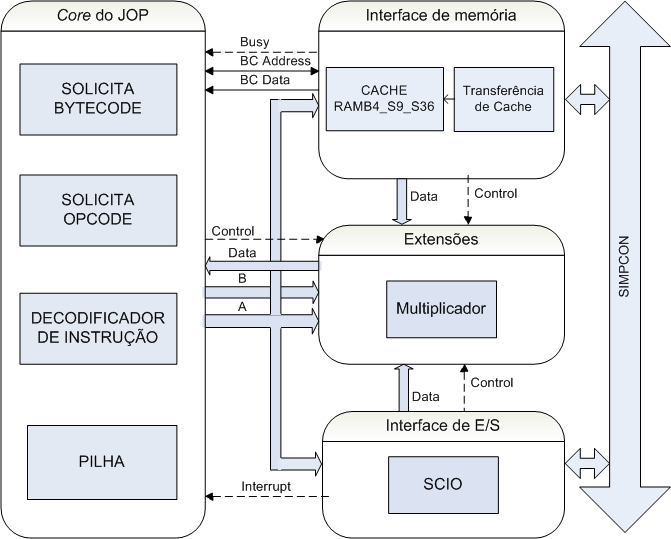
\includegraphics[width=3.0in]{arch_jop_block_port}

\caption{Diagrama de Blocos do JOP}
\label{bdjop}

\end{figure}
\subsection{Documentação e portabilidade}	
	Além das características técnicas do JOP, descritas anteriormente, podemos destacar também a ampla documentação disponível, a sua portabilidade, pois já foi implementado em diversas placas de desenvolvimento de FPGA (Xilinx e Altera) disponíveis no mercado, e por último, mas não menos importante, a disponibilidade do código fonte do JOP para \emph{download} pelo \emph{site} \url {http://www.opencores.org} e licenciado sob a GPL (\emph{Gnu Public License}) versão 3.
 Atualmente o JOP é utilizado em dois sistemas comerciais, tendo um deles a característica de tempo real, e em vários sistemas de pesquisa \cite{jop:jnl:jsa2007}. Portanto, o JOP se posiciona como uma excelente alternativa para plataforma base, de pesquisa e desenvolvimento, de novas técnicas de sistemas de tempo real.
\section{JOP Tolerante a Falhas}
	Erros na memória de código de um sistema computacional são críticos por serem armazenados permanentemente e podem, portanto, causar sucessivos erros no processo de computação que fizer uso dos dados errôneos. Para detectar e corrigir erros na memória de dados, existem técnicas bastante efetivas implementadas em \emph{software}. No entanto, as técnicas aplicadas no âmbito de \emph{software} para detectar e corrigir erros na memória de código não são eficazes, pois o próprio \emph{software} pode estar corrompido. Nesse sentido, propomos o uso de uma técnica no âmbito de \emph{hardware} para detectar e corrigir erros nas memórias RAM interna (\emph{cache}) ao processador JOP, de forma a aumentar a confiabilidade do sistema de \emph{cache} de métodos descritos na seção anterior.

	Durante a inicialização do processador JOP, todo o código é transferido da memória \emph{flash} para a memória RAM. Ao fim da transferência de código para a RAM, o sistema de \emph{cache} transferirá, sob demanda, métodos inteiros da memória externa para a memória de \emph{cache} interna. Por último, após o método estar completamente carregado na memória interna, o \emph{core} irá solicitar e executar os \emph{bytecodes}, um a um.

	A Figura \ref{jopmodificado} mostra o diagrama de blocos do JOP modificado. Quando comparado ao diagrama de blocos do JOP original (ver Figura \ref{bdjop}), nota-se que três novos blocos foram adicionados ao bloco  de interface de memória da arquitetura original  do JOP. Estes blocos se referem à implementação da técnica de proteção de ins\-tru\-ções:
\begin{enumerate}
\item Codificador de Hamming;
\item Detector e corretor de erros em bytecodes (Decodificador de Hamming);
\item Redundância de cache (RAMB4\underline{ }S4\underline{ }S18);
\end{enumerate}


\begin{figure}[!t]
\centering
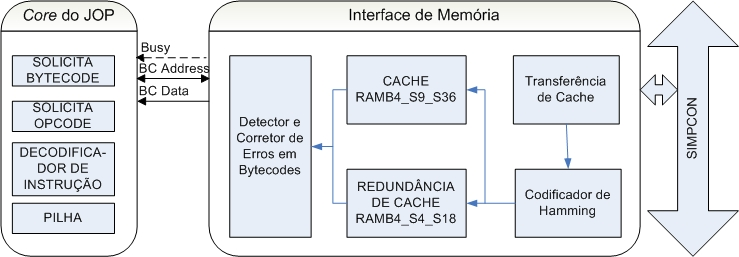
\includegraphics[width=3.0in]{jopmodificado_port}
\caption{Diagrama de Blocos do JOP modificado}
\label{jopmodificado}
\end{figure}	

\subsection{Técnica de proteção de instruções}
	Esta técnica detecta e corrige erros ocorridos nos \emph{bytecodes}, desde o armazenamento destes na \emph{cache} até o início da execução destes pelo \emph{core} do JOP. O erro é detectado e corrigido imediatamente antes de o \emph{core} iniciar a exe\-cu\-ção do \emph{bytecode}. Portanto, essa é uma técnica de verificação de último instante (\emph{last minute check})\cite{helanothesis}.
	
	Simultaneamente à escrita de um \emph{bytecode} (tamanho de 8 bits) na memória \emph{cache}, 4 bits extras de redundância (bits de Hamming) são calculados e armazenados em uma memória \emph{cache} de redundância (ver Figura \ref{jopmodificado}), que se posiciona em paralelo com a \emph{cache} original. Esses bits extras são calculados por um \emph{core} escrito em RTL (\emph{Register Transfer Level}), que implementa um codificador de Hamming.

	Imediatamente após a memória \emph{cache} fornecer um \emph{bytecode} para o \emph{core} do JOP, porém antes de ser executado, um \emph{core} decodificador de Hamming lê os 4 bits armazenados na \emph{cache} de redundância (Ver Figura \ref{jopmodificado}). Com base nesses 12 (doze) bits (oito bits do \emph{bytecode} mais quatro bits de Hamming), esse \emph{core} irá verificar se houve alguma inversão de bit em algum dos bits do \emph{bytecode}. Em caso afirmativo, isto significa que houve uma falha. Neste caso, o \emph{core} decodificador de Hamming irá corrigir automaticamente o \emph{bytecode}, desde que apenas um bit tenha sido invertido. Finalmente, o \emph{bytecode} correto será entregue para a execução por parte do \emph{core} do JOP.
	
\subsection{Percepção da falha no âmbito sistêmico}
	Uma falha de \emph{hardware} no JOP original, como por exemplo, um \emph{opcode} ilegal, leva o sistema a um \emph{shutdown} \cite{JopHandbook}. Neste trabalho, o processador foi modificado para que, na ocorrência de uma falha de \emph{hardware}, uma exceção seja gerada.
\verbatiminput{exception}

\section{Resultados}
	O JOP modificado pelo uso da técnica de proteção de ins\-tru\-ções foi simulado utilizando a ferramenta NC-VHDL para avaliar se houve regressão de seu funcionamento. Para avaliar a eficácia da técnica foi desenvolvido um módulo injetor de falhas escrito em VHDL. Esse módulo gera aleatoriamente eventos do tipo SEU nos BYTECODES de um programa em execução pelo JOP, sendo que não deve existir mais que um dos bits invertidos em um mesmo BYTECODE. A técnica mostrou-se eficaz, tendo em vista que todos os bytecodes corrompidos com somente um bit invertido, foram automaticamente corrigidos. Para aqueles com dois bits invertidos, uma exceção foi gerada para ser tratada por rotina específica para este fim.
	Além da simulação, o JOP modificado foi embarcado na placa Spartan-3 starter kit board \cite{ug130} da Digilent. Essa placa contém uma FPGA Spartan 2 XC3S200 e 1MB de memória SRAM. Neste caso, a injeção de falhas foi realizada através de mudanças do nível lógico dos pinos da FPGA. Dois tipos de falhas foram injetadas: stuck-at (1 ou 0) e inversão de bits aleatórios. Para todas as falhas inseridas, de um tipo ou de outro, houve detecção e correção automática pelo uso da técnica de proteção de instruções. Em termos numéricos, a possibilidade de detecção de falhas pode ser facilmente caculada com base no algoritimo de hamming aplicado a 8 bits de dados úteis e 4 bits de redundância \cite{shoomanbook}.

	A Tabela \ref{tabela_resultados} compara a área de FPGA, em termos de \emph{slices} e de memória RAM para o JOP original e o JOP modificado (JOPFT) pela técnica proposta.
\begin{table}[!t]
%% increase table row spacing, adjust to taste
\renewcommand{\arraystretch}{1.3}
% if using array.sty, it might be a good idea to tweak the value of
% \extrarowheight as needed to properly center the text within the cells
\caption{Tabela Comparativa entre o JOP Modificado e o JOP Original}
\label{tabela_resultados}
% Some packages, such as MDW tools, offer better commands for making tables
% than the plain LaTeX2e tabular which is used here.
\begin{tabular}{|c|c|c|c|}
	\hline
 &  FPGA Slices    &   RAM   (Kbits)   & Freq   (MHz)   \\
	\hline
JOP   & 3150 & 16 & 100  \\ 	\hline
JOPFT   & 3201 & 24 & 100\\ 	\hline
\end{tabular}
\end {table}
\section{Conclusão}
	De acordo com a pesquisa bibliográfica realizada, não foi encontrado nenhum processador Java que tenha simultaneamente garantia de tempo real e de funcionamento. Portanto, este trabalho é único no sentido de conceber, a partir do JOP, um processador Java de tempo real tolerante a falhas. Estas características são importantíssimas para sistemas embarcados de tempo real para aplicações que envolvem risco de vidas humanas.

	A técnica proposta utiliza algoritmo de hamming implementado em hardware para aumentar a confiabilidade do processador Java. 4 bits de Hamming são armazenados em conjunto com cada bytecode Java (palavra de 8 bits) do processador JOP.  Estes 4 bits são usados para detectar e corrigir erros na memória de código. Desta forma, agregamos ao processador JOP a capacidade de detectar e corrigir erros na memória de código. Isto permite manufaturar o JOPFT utilizando-se os mesmos processos de fabricação de silício, que são utilizados para fabricar chips comerciais, ao invés de usar processos de fabricação específicos para chips tolerantes a radiação. Logo, reduz-se drasticamente o custo por área de silício.


	Finalmente é importante destacar que proteger a memória de código do JOP é um passo importante para aumentar sua confiabilidade. Outras técnicas, como a técnica de votação de CRC de frames,  anteriomente proposta pelos autores em \cite{CRCFpga} e também as técnicas propostas em \cite{leon3ft} estão sendo aplicadas ao JOP e avaliadas em termos de confiabilidade, custo adicional em termos de área de silício, desempenho e implicações na características de tempo real do JOP, assim como foi feito para a técnica descrita neste trabalho. Portanto, como trabalho futuro, JOP modificado será testado com esta e outras técnicas de tolerância a falhas.  Destacamos ainda que esse trabalho foi aprovado para ser manufaturado na tecnologia CMOS IBM 130 nm gratuitamente no service Mosis. Portanto, o JOP modificado será prototipado no processo IBM 130 nm, para então ser submetido a testes de funcionamento quando sob bombardeamento de partículas altamente energizadas. Estes testes permitirão avaliar a confiabilidade do processador e poderão ser realizados, por exemplo, no LIN - Laboratório de Instrumentação Nuclear da UFRJ.


\section*{Agradecimentos}
	Os autores gostariam de agradecer a Funcap pelo suporte financeiro através do seu programa de bolsas de mestrado (Processo BMD0008-00052.01.05). Agradecemos também o Ministério da Ciência e Tecnologia (MCT) do Brasil, a Sociedade Brasileira de Microeletrônica (SBMICRO), a Cadence e a Anacom que viabilizaram o programa universitário da Cadence no Brasil. Agradecer ainda a Xilinx pelo apoio fornecido através de seu programa universitário. Agradecer também o Mosis, IBM e ARM que viabilizarão a manufatura do circuito integrado fruto deste trabalho. E ainda o DETI, FCPC, LESC, Flextronics Institute of Technology (FIT) e Flextronics por apoiarem este trabalho. E por último, mas não menos importante, a Martin Schoeberl por distribuir livremente o código fonte do JOP sob a licença GPL.








%-------------------------------------------------------------------------
%\nocite{ex1,ex2}
\bibliographystyle{wscad2009}
\bibliography{../rjns/biblio}
%\bibliography{wscad2009}

\end{document}

